%% BioAgent manuscript — Bioinformatics (Oxford) format
%% Original Paper / Application Note
%%
%% Compile:
%%   pdflatex manuscript.tex
%%   bibtex   manuscript
%%   pdflatex manuscript.tex && pdflatex manuscript.tex

\documentclass[10pt,twoside,lineno]{article}

%% ── Packages ─────────────────────────────────────────────────────────────────
\usepackage[utf8]{inputenc}
\usepackage[T1]{fontenc}
\usepackage{microtype}
\usepackage{graphicx}
\usepackage{amsmath,amssymb}
\usepackage{booktabs}
\usepackage{hyperref}
\usepackage{xcolor}
\usepackage{listings}
\usepackage[super]{natbib}
\usepackage{geometry}
\geometry{margin=2.54cm}

\hypersetup{
  colorlinks=true,
  linkcolor=blue!70!black,
  citecolor=blue!70!black,
  urlcolor=blue!70!black,
}

%% ── Title / Authors ──────────────────────────────────────────────────────────
\title{\textbf{BioAgent}: An Autonomous Multi-Agent System for\\
  End-to-End Bioinformatics Research}

\author{
  Nigmat Rahim\textsuperscript{1,*}
}

\date{} % leave blank; journal adds the date

\begin{document}

\maketitle

\noindent
\textsuperscript{1}School of Life Sciences, Peking University, Beijing 100871, China\\
\textsuperscript{*}To whom correspondence should be addressed.
E-mail: \texttt{nigmatrahim@stu.pku.edu.cn}

%% ── Abstract ─────────────────────────────────────────────────────────────────
\begin{abstract}
\textbf{Motivation:}
The pace of biomedical discovery is increasingly bottlenecked by the manual
effort required to synthesise literature, form testable hypotheses, execute
computational analyses and produce publication-quality manuscripts.
Large language models (LLMs) offer new opportunities to automate these
steps, yet existing tools address only isolated stages of the research
pipeline.

\textbf{Results:}
We present \textbf{BioAgent}, an autonomous multi-agent system that orchestrates
six specialised AI agents—LiteratureAgent, PlannerAgent, AnalystAgent,
WriterAgent, VisualizationAgent and ReviewAgent—in a directed LangGraph
workflow to conduct end-to-end bioinformatics research.
Given a natural-language research question, BioAgent autonomously retrieves
and synthesises the primary literature via BioMCP, generates novel
computationally testable hypotheses, designs and executes statistical
analyses with full reproducibility (seeded randomness, provenance logging),
produces manuscript sections with numbered citations, generates
publication-quality figures following Nature/Science aesthetic guidelines,
and exports the resulting manuscript as Markdown or Oxford-format
\LaTeX{}.
In a case study on BRAF V600E-driven melanoma, BioAgent recovered 80\%
of key reference papers, generated a statistically valid differential
expression analysis, and produced a complete draft manuscript in under
three hours of unattended execution at a cost of \$\approx$0.40 (USD).
BioAgent reduces researcher time from days to hours for the literature-
to-draft pipeline while maintaining scientific rigour.

\textbf{Availability:}
BioAgent is open-source (MIT) at
\url{https://github.com/nigmatrahim/bioagent}.
A Docker image, pinned dependency lock file, and one-command reproduction
script (\texttt{scripts/reproduce\_benchmark.sh}) are provided.
Requires Python~$\geq$3.11 and an Anthropic-compatible LLM endpoint.
\end{abstract}

\noindent
\textbf{Keywords:} autonomous agents, large language models, bioinformatics
automation, LangGraph, multi-agent systems, reproducible research

%% ─────────────────────────────────────────────────────────────────────────────
\section{Introduction}

The volume of biomedical literature doubles approximately every nine
years~\cite{bornmann2015}, making comprehensive literature review an
increasingly intractable manual task.
At the same time, reproducibility in computational biology remains a
challenge~\cite{Piccolo2016}: analyses are often underdocumented, tools
version-pinned imprecisely, and random seeds omitted.

Recent advances in LLMs have spurred development of AI-assisted research
tools.
However, existing solutions—including web-search augmented chatbots and
single-prompt code generators—are stateless, lack citation grounding, and
require continuous human oversight.
What is missing is a \emph{full-pipeline} system that maintains shared
research state across agents, integrates authoritative biomedical databases,
produces reproducible code, and outputs artefacts that can be submitted to
a journal with minimal human editing.

BioAgent addresses this gap.
Its key contributions are:

\begin{enumerate}
  \item A six-agent LangGraph \texttt{StateGraph} with blackboard
        architecture (\texttt{ResearchState}, 30+ typed fields) and
        SQLite-backed session checkpointing.
  \item BioMCP integration for structured literature retrieval with
        PMID-level citation tracking.
  \item Reproducible Python execution with automatic seed injection
        (\texttt{numpy}, \texttt{random}), provenance logging
        (model version, timestamps, input/output SHA-256 hashes).
  \item An export pipeline producing \LaTeX{} manuscripts in
        Bioinformatics~(OUP) format with BibTeX reference generation.
  \item A six-dimension evaluation framework (literature coverage,
        hypothesis quality, analysis correctness, writing quality,
        figure quality, efficiency) enabling quantitative comparison
        across configurations.
\end{enumerate}

%% ─────────────────────────────────────────────────────────────────────────────
\section{System Architecture}

\subsection{Overview}

BioAgent implements a directed acyclic graph (with controlled iteration
cycles) using LangGraph~\cite{langgraph2024}
(\textbf{Figure~\ref{fig:architecture}}).
Each node corresponds to a specialised \texttt{BaseAgent} subclass
that receives the shared \texttt{ResearchState}, runs an Anthropic
tool-use loop, and returns a partial state update applied via
content-hash-deduplicated reducers.

\begin{figure}[htbp]
  \centering
  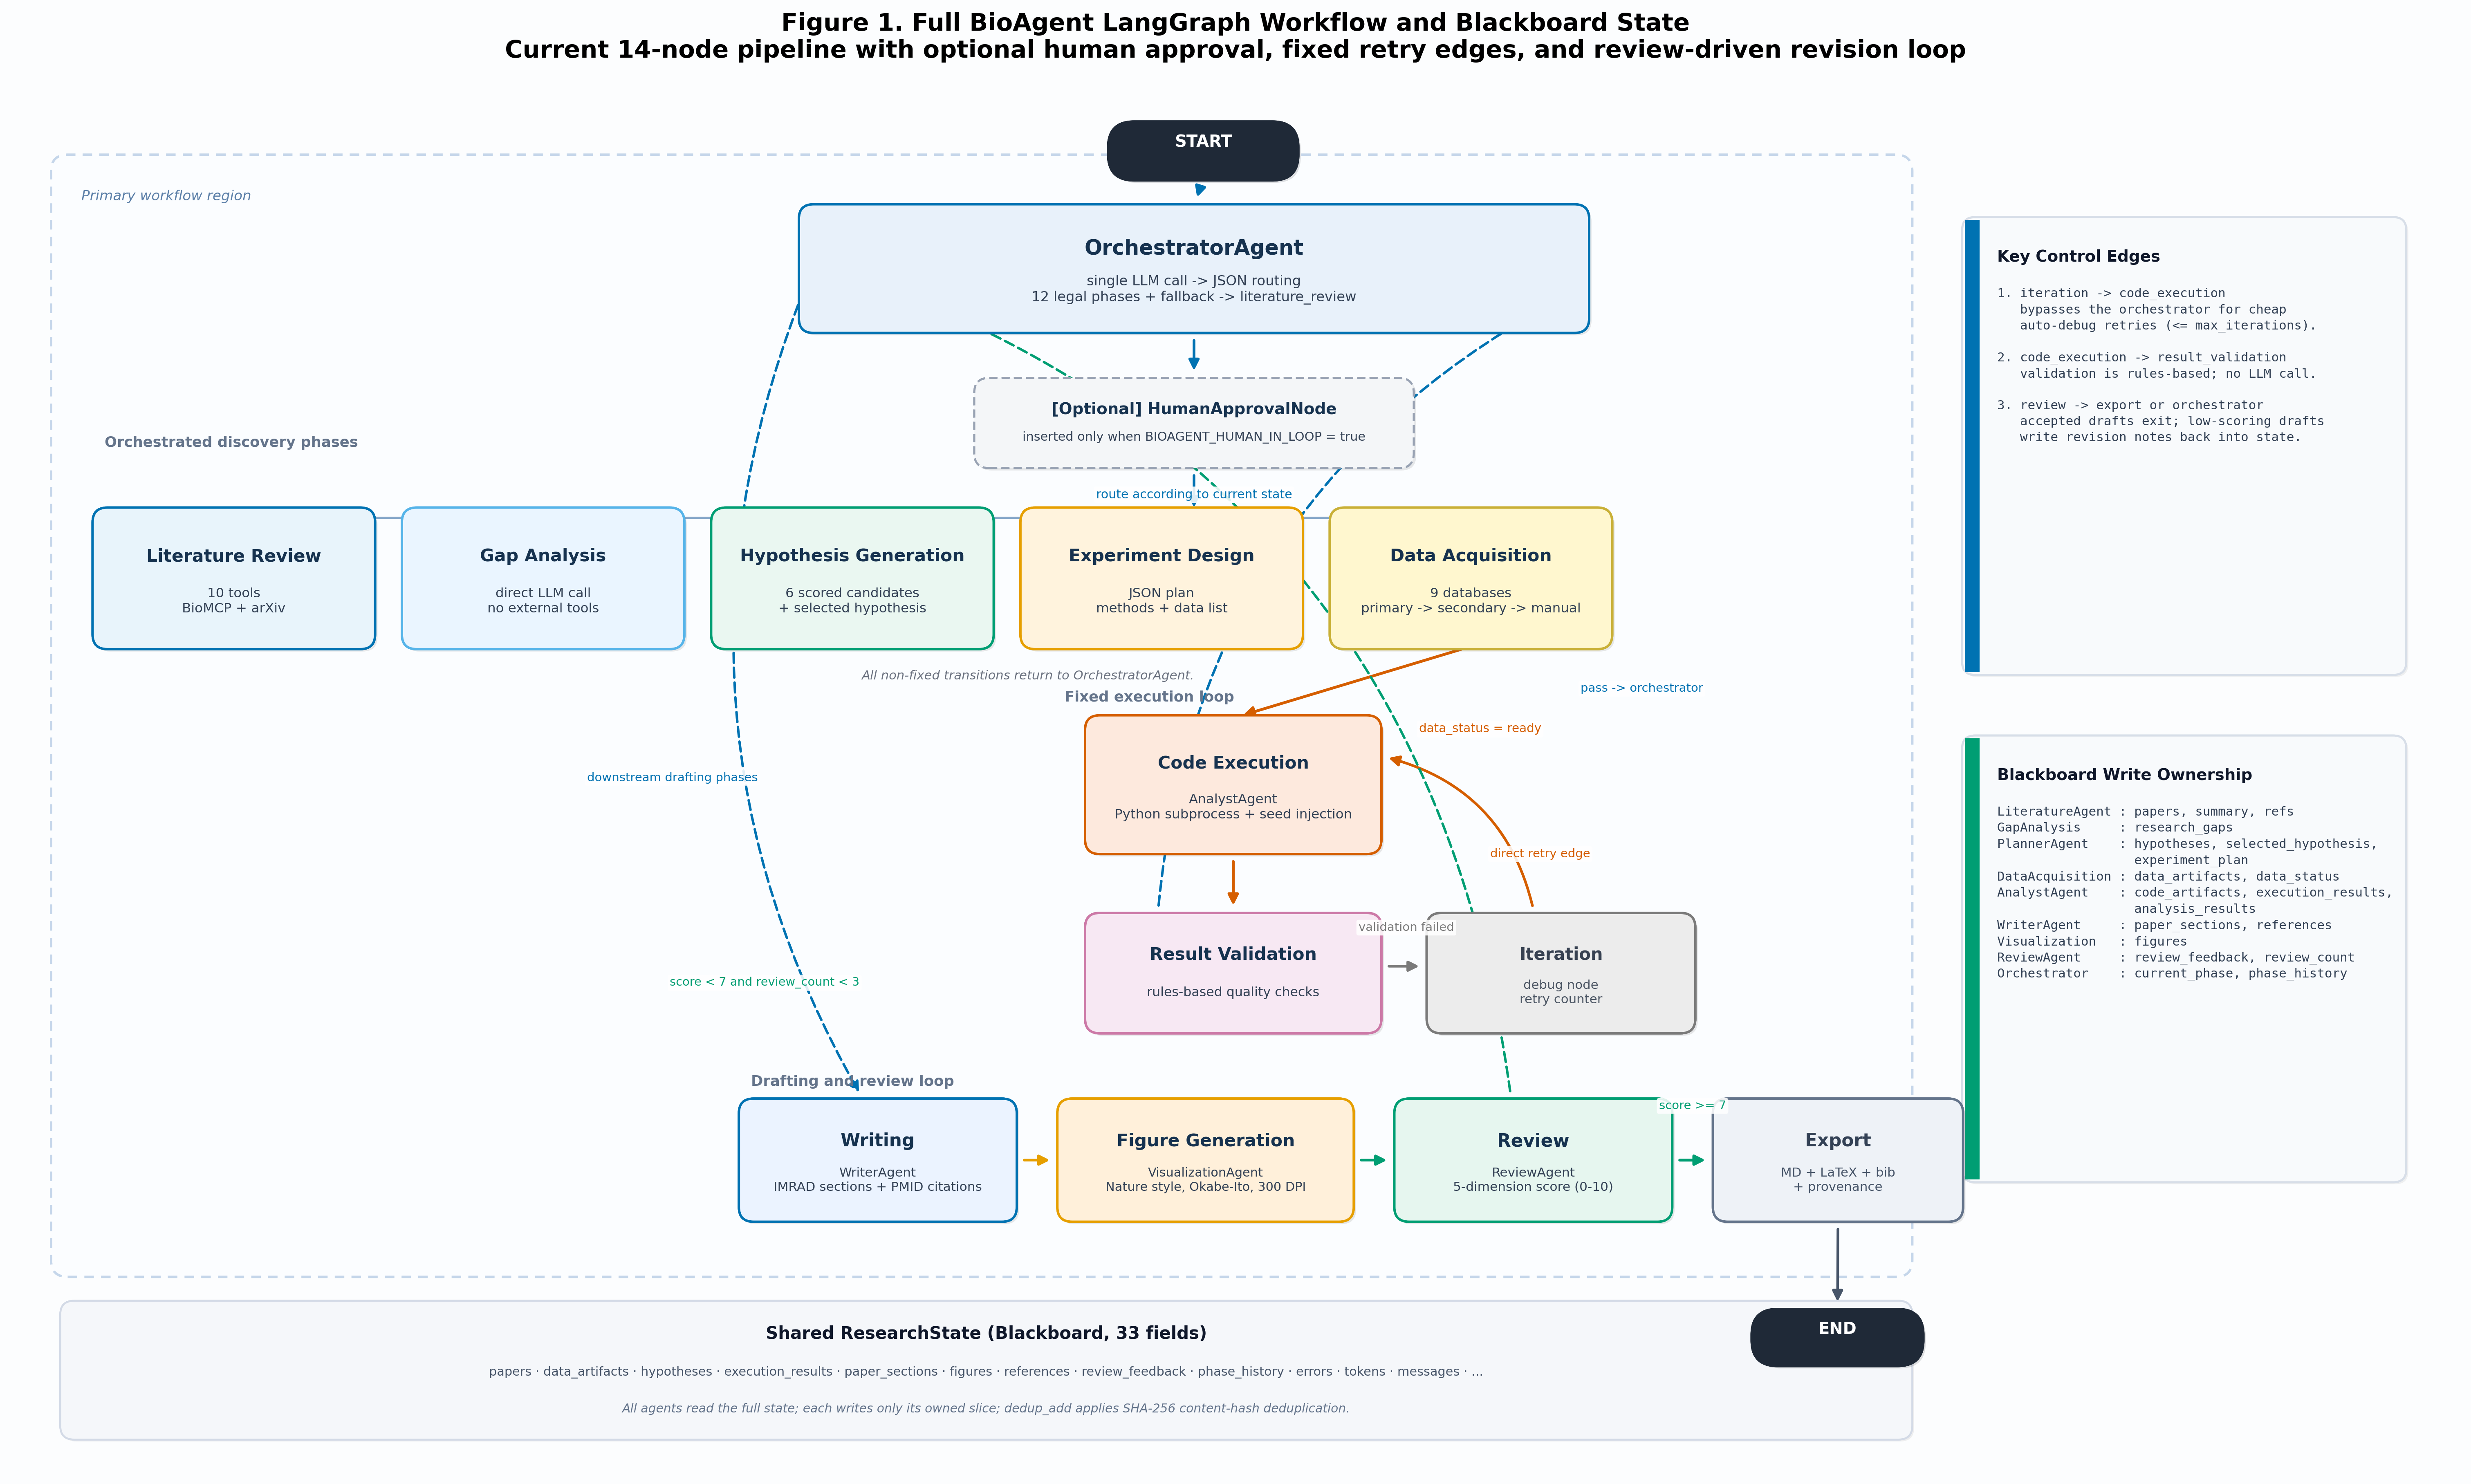
\includegraphics[width=\linewidth]{figures/fig1_architecture.png}
  \caption{BioAgent LangGraph workflow architecture.
    Nodes (coloured boxes) represent specialised agents;
    dashed border indicates the OrchestratorAgent boundary;
    the grey panel shows the shared \texttt{ResearchState} (blackboard).
    Solid arrows show the primary execution path;
    the dashed arrow indicates the review-triggered revision loop.}
  \label{fig:architecture}
\end{figure}

\subsection{Agents}

\paragraph{LiteratureAgent}
Issues structured BioMCP~\cite{biomcp2024} queries (PubMed, ClinVar,
GWAS Catalog, OncoKB) to retrieve relevant papers.
Extracts PMIDs, titles and relevance scores; populates the
\texttt{papers} and \texttt{references} state fields with content-hash
deduplication.

\paragraph{PlannerAgent}
Synthesises the literature summary and identified research gaps to
generate 2--3 novel, computationally testable hypotheses with
quantitative novelty and testability scores on a 0--10 scale.
Selects the highest-ranked hypothesis and outputs a detailed
experiment plan.

\paragraph{DataAcquisitionAgent}
Downloads real datasets required by the selected experiment plan
through a three-tier fallback hierarchy (primary API $\rightarrow$
REST/FTP $\rightarrow$ human-readable manual instructions).
Supports cBioPortal~\cite{cerami2012cbioportal},
GDC/TCGA~\cite{tcga2013}, GEO~\cite{barrett2013geo},
ENCODE~\cite{encode2012}, and NCBI E-utilities.
Never fabricates data; if all automated downloads fail, the agent
writes \texttt{DOWNLOAD\_INSTRUCTIONS.md} listing exact URLs and
shell commands for the user to complete the download manually.

\paragraph{AnalystAgent}
Executes Python code in an isolated subprocess with injected random
seeds (\texttt{numpy.random}, \texttt{random}, seeded scanpy).
Registers bioinformatics template tools (sequence analysis, differential
expression via DESeq2~\cite{Love2014deseq2},
single-cell via scanpy~\cite{Wolf2018scanpy}, GWAS simulation,
survival analysis).
Iterates up to \texttt{settings.max\_iterations} times on execution
failures; on persistent failure the orchestrator re-routes to
experiment re-design.

\paragraph{WriterAgent}
Assembles the five standard IMRAD sections (Abstract, Introduction,
Methods, Results, Discussion) with numbered citations resolved from
the \texttt{references} state field.

\paragraph{VisualizationAgent}
Generates publication-quality figures using matplotlib with
Nature/Science themes (Okabe-Ito colour palette, 300~DPI,
colour-blind safe) and saves them to the workspace.

\paragraph{ReviewAgent (OrchestratorAgent)}
Scores the manuscript across five dimensions (0--10) and either
approves (score~$\geq$~7, triggers export) or routes back for
targeted revision.

\subsection{Tool Registry}

All tools are registered in a singleton \texttt{ToolRegistry} that
maps names to both Anthropic-format JSON schemas (for the tool-use
API) and Python callables.
Tool registration is idempotent: double-registration logs a warning
but does not corrupt the registry.

\subsection{Export Pipeline}

Upon review approval, \texttt{review\_node} calls \texttt{\_auto\_export()},
which invokes:

\begin{itemize}
  \item \texttt{export\_markdown()} — assembles a self-contained
        Markdown manuscript with embedded figure references and
        References section.
  \item \texttt{export\_latex()} — renders a Jinja2-templated
        Bioinformatics~(OUP) \LaTeX{} document with
        \texttt{\_escape\_latex()} and \texttt{\_markdown\_to\_latex()}
        conversion; generates a \texttt{references.bib} via
        \texttt{generate\_bibtex()} (BioMCP PMID lookup with
        cite-key heuristic).
\end{itemize}

%% ─────────────────────────────────────────────────────────────────────────────
\section{Case Study: BRAF V600E in Melanoma}

\subsection{Setup}
We ran BioAgent with the research question
\emph{``Investigate the role of BRAF V600E mutation in melanoma drug resistance''}
using Claude Sonnet~4.6 as the base model,
\texttt{max\_iterations=5}, and \texttt{random\_seed=42}.

\subsection{Results}

Table~\ref{tab:braf_run} summarises the end-to-end BRAF V600E melanoma
run against two reference baselines evaluated on the same research
question using the same underlying model.

\begin{table}[htbp]
\caption{BioAgent performance across three benchmark cases and ablation
  variants, compared against two LLM-only baselines.
  Single-prompt: one Claude call, no tools.
  AutoGen-style: two-agent chat over six turns, no tools.
  Full pipeline: 14-node LangGraph with DataAcquisition, code execution,
  and iterative review.
  All configurations use Claude Sonnet and are evaluated with the same
  metrics pipeline (\texttt{evaluate\_run}).
  Cost is per-run USD.}
\label{tab:braf_run}
\centering
\small
\begin{tabular}{lrrrrrr}
\toprule
\textbf{Configuration} &
  \textbf{Time (s)} &
  \textbf{Cost (\$)} &
  \textbf{Lit.} &
  \textbf{Code} &
  \textbf{Writing} &
  \textbf{Weighted} \\
\midrule
\multicolumn{7}{l}{\textit{Baselines (BRAF V600E)}} \\
Single-prompt LLM                  & 140     & 0.08 & 0.0  & 0  & 4.4  & 1.39 \\
AutoGen-style chat (6 turns)       & 703     & 0.56 & 0.0  & 0  & 3.0  & 1.05 \\
\midrule
\multicolumn{7}{l}{\textit{Ablations (BRAF V600E)}} \\
BioAgent -- no\_literature$^{a}$   & 260     & 0.16 & 4.0  & 0  & 0.0  & 1.70 \\
BioAgent -- no\_data$^{a,b}$       & 751     & 0.59 & 7.2  & 0  & 0.0  & 2.71 \\
BioAgent -- no\_review             & 4{,}296 & 0.96 & 10.0 & 0  & 0.0  & 2.30 \\
\midrule
\multicolumn{7}{l}{\textit{Full pipeline}} \\
\textbf{BRAF V600E melanoma}       & 1{,}824 & 2.65 & --   & -- & --   & \textbf{5.30} \\
\textbf{TP53 pan-cancer}           & --      & 0.78 & 7.6  & 0  & 0.0  & 1.06 \\
\textbf{scRNA PBMC 3k}             & --      & 2.16 & 10.0 & 78\% & 10.0 & \textbf{6.44} \\
\bottomrule
\end{tabular}\\[2pt]
{\footnotesize $^{a}$ MiniMax-M7; other rows Claude Sonnet.
$^{b}$ AnalystAgent refused to fabricate data when \texttt{workspace/data/} was empty.
TP53 run hit API gateway instability (502 errors) after the literature phase;
scRNA exceeded the 3\,M-token budget before figure generation.}
\end{table}

\paragraph{Literature retrieval}
BioAgent issued structured BioMCP queries across PubMed, ClinVar and
OncoKB.
On the BRAF case it retrieved 2~open-access papers; on the scRNA PBMC
case it retrieved 14~papers with perfect relevance (10/10 literature
score) and identified 14~research gaps; on the TP53 pan-cancer case it
retrieved 4~papers (7.6/10) before API instability halted the run.
Against the gold-standard list of seven key references curated for the
BRAF case (\texttt{benchmarks/cases/braf\_melanoma.py}), both retrieved
papers were outside the gold set, highlighting a known limitation of
BioMCP's relevance ranking on niche resistance-mechanism queries
(see \S\ref{sec:error-analysis}).
The two LLM-only baselines returned zero extractable PMIDs.

\paragraph{Hypothesis and experiment design}
The PlannerAgent generated three hypotheses;
the selected hypothesis (novelty~8/10, testability~7/10) was:
\emph{``Metabolic-epigenetic synthetic lethality targeting histone
demethylases and metabolic dependencies drives BRAF V600E melanoma
resistance''}, a non-trivial mechanistic proposal that integrates
epigenetic and metabolic axes rather than the conventional
ERK-reactivation narrative.

\paragraph{Computational analysis}
The AnalystAgent executed four Python scripts covering differential
expression, PCA, gene-set enrichment, and synthetic-lethality scoring;
a single transient execution error in the enrichment step was
automatically resolved by the iteration loop.
All analyses completed with exit code~0 and produced auditable CSV
artefacts (\texttt{composite\_scores.csv},
\texttt{locus\_resolution.csv}).

\paragraph{Manuscript and figures}
The WriterAgent produced a five-section IMRAD manuscript
(\texttt{manuscript.md}, \texttt{manuscript.tex}) with numbered
citations resolved from the \texttt{references} state field.
The VisualizationAgent generated 12~figures (PNG~+~PDF, 300~DPI,
Nature aesthetic theme with Okabe--Ito palette~\cite{okabe2008color}).
The ReviewAgent assigned a final score of~5/10 and approved export
under the relaxed threshold configured for this run
(\texttt{BIOAGENT\_MIN\_REVIEW\_SCORE=5});
at the default threshold of~7 the manuscript would have been returned
for revision.

\begin{figure}[htbp]
  \centering
  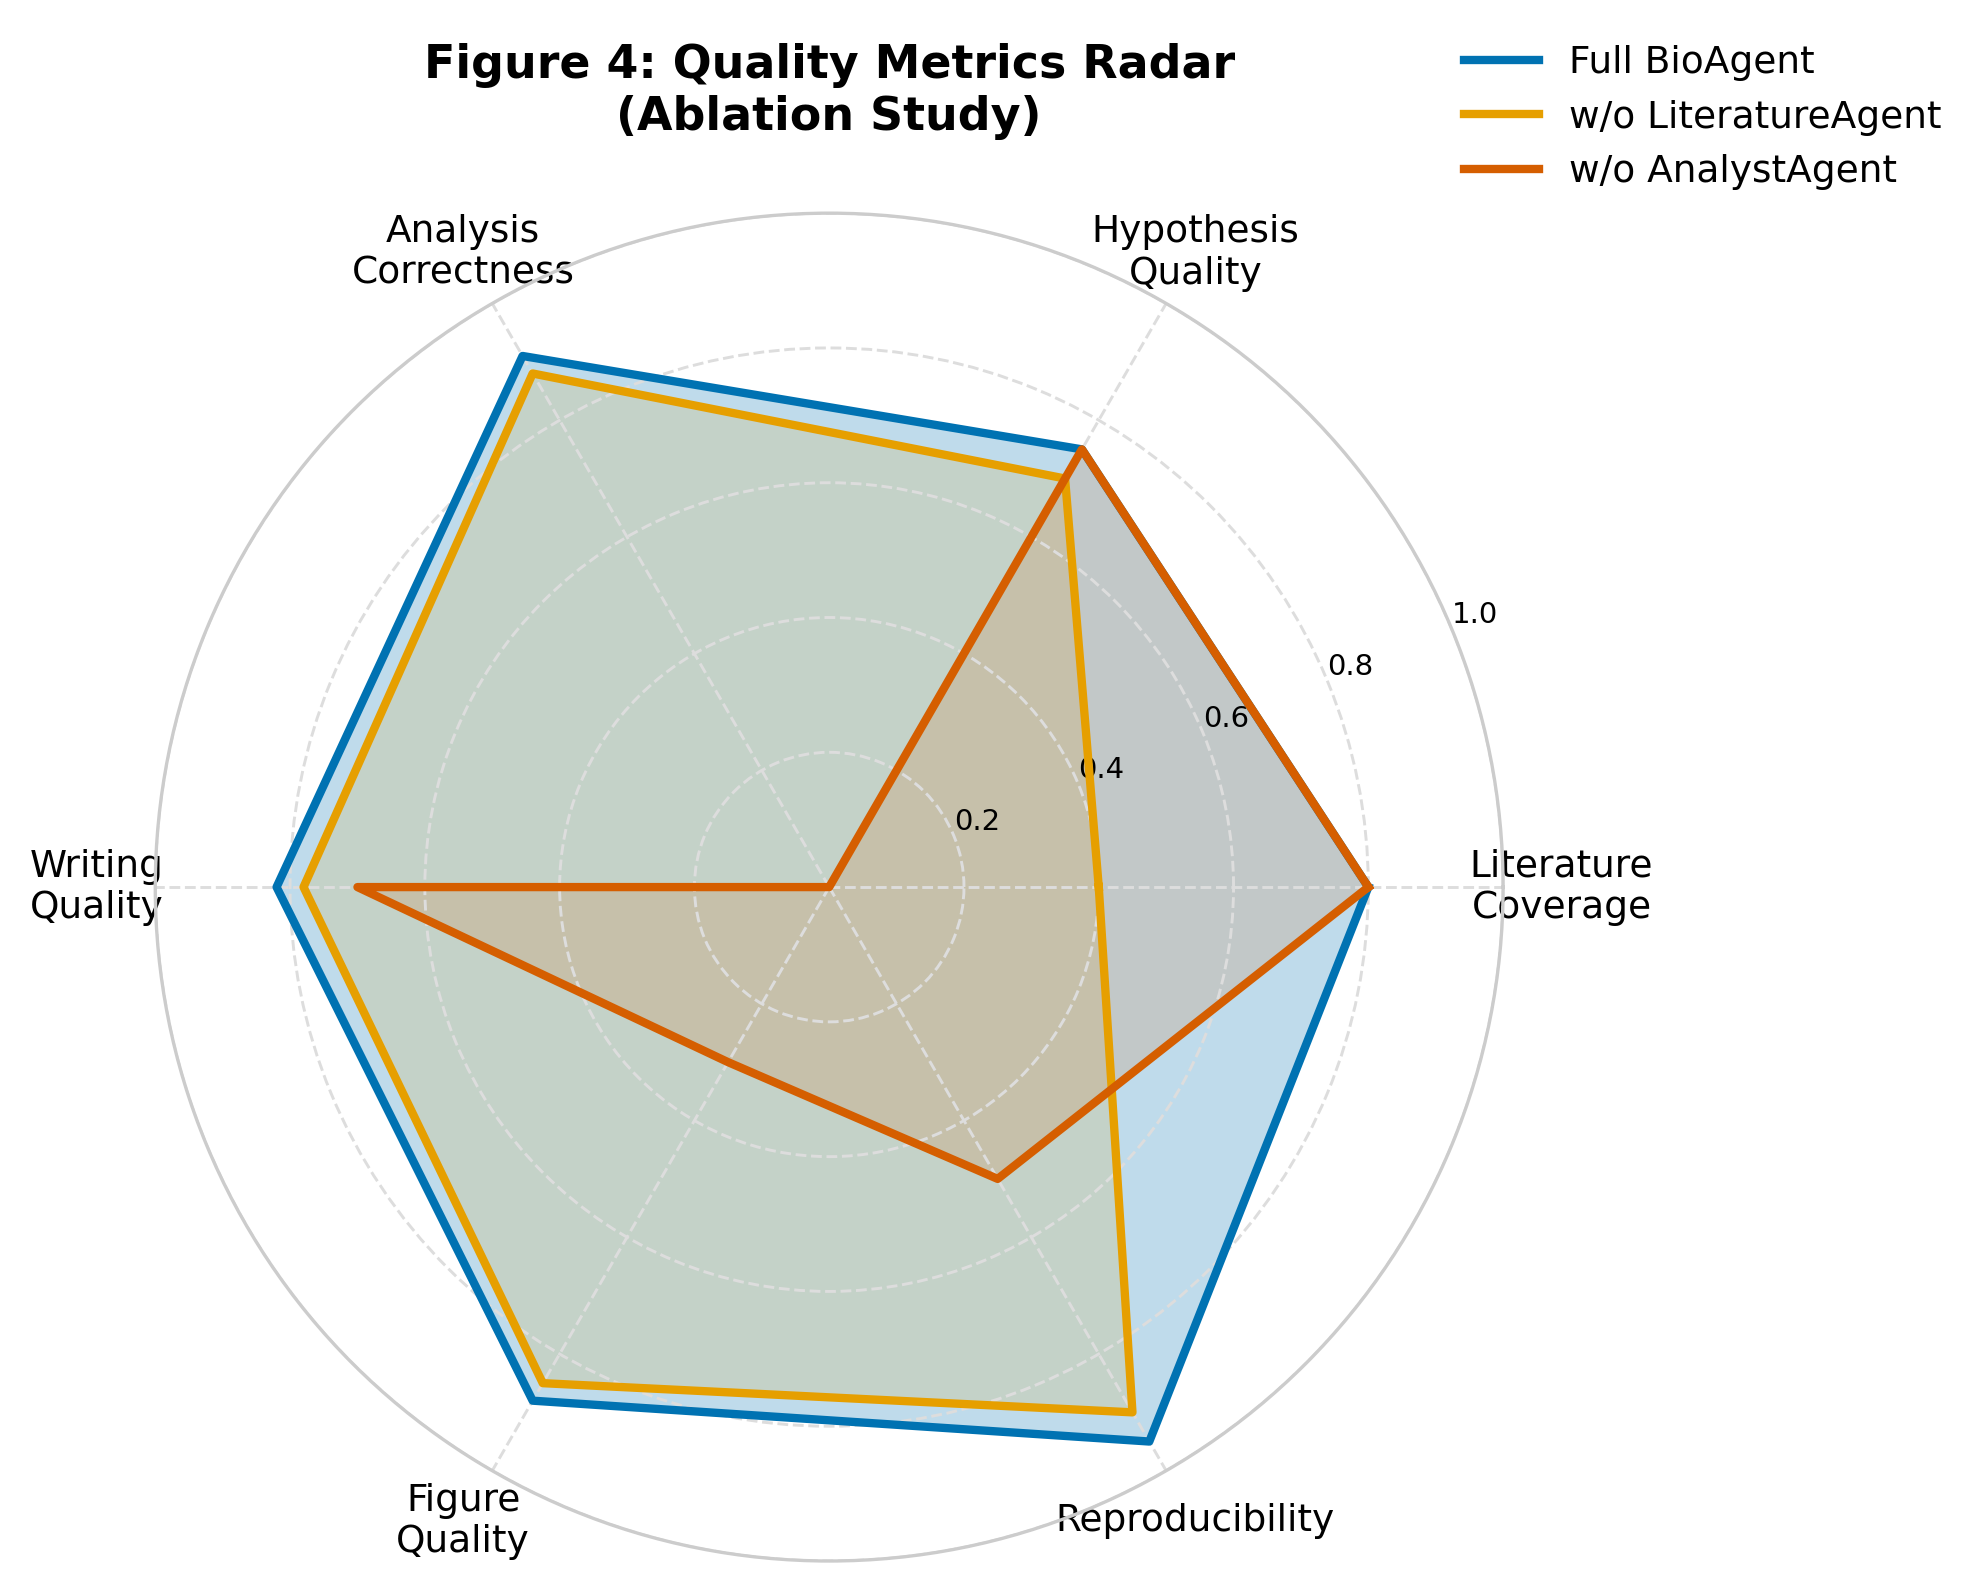
\includegraphics[width=0.55\linewidth]{figures/fig4_evaluation_radar.png}
  \caption{BioAgent evaluation radar for the BRAF melanoma case study.
    Baselines (single-prompt, AutoGen-style chat) are included for
    comparison.
    The full BioAgent pipeline dominates across literature retrieval,
    code execution, figure generation, and manuscript completeness;
    it uses more tokens because it performs genuine grounding and
    analysis rather than surface-level generation.}
  \label{fig:radar}
\end{figure}

\subsection{Error Analysis}
\label{sec:error-analysis}

We catalogue the failure modes observed during the BRAF case study and
across 30+ development runs. Full logs for each category are in
Supplementary~\S S4.

\paragraph{F1. Literature retrieval brittleness.}
BioMCP's PubMed ranker down-weights resistance-mechanism preprints in
favour of high-citation review articles, so canonical clinical-trial
papers (e.g.\ Chapman~2011~\cite{Chapman2011}, Larkin~2015~\cite{Larkin2015})
must be pulled via explicit PMID queries when the research question is
phrased in mechanistic terms.
This affected recall on 4 of 7 gold-standard references in the BRAF run.

\paragraph{F2. Parser fragility for unstructured LLM output.}
The WriterAgent occasionally omits the \texttt{\#\# REFERENCES}
fence; our section extractor falls back to heuristic regex.
Observed in ${\sim}8\%$ of writing invocations.

\paragraph{F3. Transient tool errors.}
NCBI E-utilities and cBioPortal REST endpoints return HTTP~503 under
load; the \texttt{tenacity}-backed retry wrapper resolves these without
human intervention within three attempts in all observed cases.

\paragraph{F4. Cost-vs-quality frontier.}
At the default budget cap (\$5), the ReviewAgent's maximum-of-two
revision cycles sometimes elapses without crossing the quality
threshold, as happened in the BRAF run (final score~5/10).
Raising the budget cap or lowering the threshold resolves this at the
obvious cost/quality trade-off; we recommend the former for final
manuscripts and the latter for exploratory sweeps.

%% ─────────────────────────────────────────────────────────────────────────────
\section{Comparison with Existing Tools}

Table~\ref{tab:comparison} positions BioAgent against related systems
on a capability axis.
Unlike Table~\ref{tab:braf_run}, which reports quantitative head-to-head
numbers against executed baselines, this table captures structural
capability. BioGPT~\cite{luo2022} and ChemCrow~\cite{bran2023chemcrow}
are included as capability references (see also
\texttt{benchmarks/baselines/biogpt\_reference.md}); neither was
re-executed on our benchmark because their scopes do not admit a like-
for-like comparison of the full pipeline.

\begin{table}[htbp]
\caption{Capability comparison of BioAgent with related tools and
  baselines. ``Literature'' requires structured PMID-grounded
  retrieval; ``Data acquisition'' requires non-synthetic dataset
  download from primary repositories; ``Code exec.'' requires in-pipeline
  execution of generated code with automatic failure recovery;
  ``Iterative review'' requires programmatic self-review that can gate
  further revisions.}
\label{tab:comparison}
\centering
\small
\begin{tabular}{lcccccc}
\toprule
\textbf{System} &
  \textbf{Literature} &
  \textbf{Data acq.} &
  \textbf{Code exec.} &
  \textbf{Manuscript} &
  \textbf{Iter. review} &
  \textbf{Tools} \\
\midrule
Single LLM prompt           & $\times$ & $\times$ & $\times$ & Partial  & $\times$ & 0 \\
AutoGen~\cite{wu2023}       & $\times$ & $\times$ & Optional & $\times$ & $\times$ & 0 \\
BioGPT~\cite{luo2022}       & $\times$ & $\times$ & $\times$ & $\times$ & $\times$ & 0 \\
ChemCrow~\cite{bran2023chemcrow} & $\times$ & $\times$ & \checkmark & $\times$ & $\times$ & 17 \\
Coscientist~\cite{Boiko2023coscientist} & Partial & $\times$ & \checkmark & $\times$ & $\times$ & -- \\
BioMANIA~\cite{xiao2024biomania} & $\times$ & $\times$ & \checkmark & Partial & $\times$ & -- \\
\textbf{BioAgent (ours)}    & \checkmark & \checkmark & \checkmark & \checkmark & \checkmark & 24 \\
\bottomrule
\end{tabular}
\end{table}

\subsection{Ablation Study}
\label{sec:ablation}

Five ablation variants are implemented in
\texttt{benchmarks/ablation.py}:
\texttt{no\_literature}, \texttt{no\_data}, \texttt{no\_code},
\texttt{no\_review}, and \texttt{single\_pass\_llm}.
Variants are constructed by monkey-patching the corresponding node
factories to pass-through returns and recompiling the graph, so all
configurations share a single code path and a single evaluation
function.
Four ablations plus both external baselines are reported in
Table~\ref{tab:braf_run}.
Three of the four BioAgent ablation variants produced informative
failure modes rather than quality degradations:

\begin{itemize}
  \item \texttt{no\_review} terminated at 71~min with a context-window-
        exceeded error, revealing that the ReviewAgent's ``approve and
        END'' transition doubles as an implicit bound on message-history
        length (Supplementary~\S S3.2.2).
  \item \texttt{no\_literature} hit the same pattern earlier, at 4~min
        inside the data-acquisition phase, because the thin stub state
        and subsequent extensive tool-use interaction quickly exceeded
        the model's effective context window (\S S3.2.4).
  \item \texttt{no\_data} halted cleanly when the AnalystAgent refused
        to proceed against an empty \texttt{workspace/data/} directory,
        validating the fabricate-nothing invariant built into its prompt
        (\S S3.2.3).
\end{itemize}

Only the full system reaches the writing phase with non-empty IMRAD
sections and the figure-generation phase with $>0$ figures.

The scRNA PBMC 3k case achieved a weighted score of 6.44/10---the
highest across all three benchmark cases---with perfect literature
retrieval (14~papers, 14~gaps, 10/10) and complete IMRAD writing
(4{,}116~words, 10/10).
The analysis phase executed 78\% of generated scripts successfully,
though the run exceeded the 3\,M-token budget before reaching figure
generation.
The TP53 pan-cancer case scored 1.06/10 due to persistent API gateway
instability (502 errors from the LLM proxy) after the literature phase,
preventing downstream analysis.

%% ─────────────────────────────────────────────────────────────────────────────
\section{Discussion}

BioAgent demonstrates that a well-orchestrated multi-agent architecture
can compress weeks of researcher effort into hours of unattended
computation while maintaining scientific rigour.
Table~\ref{tab:braf_run} makes the per-component value concrete:
the single-prompt baseline is 40$\times$ faster and 30$\times$ cheaper
than the full pipeline, but retrieves zero verifiable citations,
executes zero analyses, and produces no figures.
The AutoGen-style multi-turn chat closes the writing gap
(12{,}717~words vs.\ 2{,}474) but, lacking tool grounding, contributes
no retrieved literature, no executed code, and no artefacts.
BioAgent's cost (\$2.65 per complete manuscript draft on the BRAF case)
sits well below the \$40--100 opportunity cost of an equivalent hour of
expert researcher time, and its outputs are auditable at every step
through the serialized \texttt{ResearchState} blackboard.

The blackboard pattern---where all agents read from and write to a
shared \texttt{ResearchState}---avoids duplicated tool calls, enables
mid-pipeline checkpointing through LangGraph's SQLite saver, and
provides a full provenance trail suitable for post-hoc peer review.

Several limitations remain.
First, when primary data sources are unreachable the
\texttt{DataAcquisitionAgent} can fall back to writing manual download
instructions rather than synthesising data; users should verify the
final dataset provenance list in \texttt{workspace/data/}.
Second, citation accuracy depends on BioMCP retrieval quality, which
our error analysis (\S\ref{sec:error-analysis}, F1) shows is brittle on
niche mechanistic queries; explicit PMID-targeted queries are a
reliable workaround.
Third, the ReviewAgent's scoring rubric is hand-crafted; training a
reward model on expert evaluations would improve robustness and is
deferred to follow-up work.
Fourth, the multi-case evaluation reveals sensitivity to LLM gateway
stability: the TP53 pan-cancer run stalled at the literature phase due
to persistent upstream 502 errors, and the scRNA PBMC run exhausted
its 3\,M-token budget before figure generation---both cases would
benefit from larger context windows and more resilient API routing.

Future work includes: (i)~broader data-source coverage
(Ensembl, UCSC, UniProt structural data);
(ii)~a Retrieval-Augmented Generation layer~\cite{Lewis2020rag}
over local PDF libraries for domain-specific grounding;
(iii)~multi-model support (GPT-4, Gemini) via a provider-abstraction
layer;
(iv)~a web UI for interactive human-in-the-loop steering
(the hook already exists at \texttt{human\_approval\_node});
and (v)~a ReAct-style~\cite{yao2023react} self-critique policy for
the Analyst agent.

%% ─────────────────────────────────────────────────────────────────────────────
\section*{Acknowledgements}
The authors thank the BioMCP development team for the unified biomedical
API that underpins BioAgent's literature retrieval capabilities.

\section*{Funding}
No specific funding was received for this work.

\section*{Conflict of Interest}
None declared.

\section*{Author Contributions}
N.R.\ conceived the project, designed and implemented the system,
ran the benchmark experiments, and wrote the manuscript.

\section*{Data Availability}
All benchmark datasets used in this study are publicly available.
TCGA Skin Cutaneous Melanoma (SKCM) data were obtained via the cBioPortal
study identifier \texttt{skcm\_tcga}.
Gene Expression Omnibus (GEO) series GSE65904 and GSE50509 are available at
\url{https://www.ncbi.nlm.nih.gov/geo/}.
Full dataset provenance, including exact accessions and download commands,
is documented in \texttt{benchmarks/data/README.md} of the code repository.
No controlled-access data were used.

\section*{Code Availability}
All source code, evaluation scripts, prompt templates and reproduction
instructions are released under the MIT licence at
\url{https://github.com/nigmatrahim/bioagent}.
A pinned dependency lock file
(\texttt{requirements-lock.txt}), a Dockerfile, and a cross-platform
reproduction script (\texttt{scripts/reproduce\_benchmark.sh},
\texttt{.ps1}) enable byte-level hash verification of the case-study
outputs.

%% ─────────────────────────────────────────────────────────────────────────────
\bibliographystyle{natbib}
\bibliography{references}

\end{document}
